\documentclass[11pt]{article}

\usepackage{fullpage,times}%charter}
\usepackage{color}

\usepackage{tikz}
\usetikzlibrary{arrows.meta}

%% macros
\newcommand{\ax}[1]{\texttt{AX}(#1)}
\newcommand{\ex}[1]{\texttt{EX}(#1)}
\newcommand{\af}[1]{\texttt{AF}(#1)}
\newcommand{\ef}[1]{\texttt{EF}(#1)}
\newcommand{\ag}[1]{\texttt{AG}(#1)}
\newcommand{\eg}[1]{\texttt{EG}(#1)}
\newcommand{\au}[2]{\texttt{A}(#1\ \texttt{U}\ #2)}
\newcommand{\eu}[2]{\texttt{E}(#1\ \texttt{U}\ #2)}
\newcommand{\sem}[1]{[\!\![#1]\!\!]}

\newcommand{\sol}[1]{{\color{blue}#1}}

\begin{document}

\hrule
\smallskip

\noindent
\emph{Please review and study the solutions for homework assignment 1
before proceeding with this assignment. }

\noindent
You can review the latex source for this assignment-file to
learn and use latex to prepare your homework submission. You will see
the use of macros (to write uniformly formatted text), different
text-styles (emphasized, bold-font), different environments (figures,
enumerations).

It is not required that you use exactly this latex source to prepare
your submission. 
\smallskip
\hrule


\begin{center}
{\Large\bf Homework 2 (CTL): ComS/CprE/SE 412, ComS 512}

\medskip

Due-date: Feb 17 at 11:59PM.

\medskip


\end{center}

\noindent
\textbf{
Submit online on Canvas two files: the source file in latex format and
the pdf file generated from latex. Name your files:
$\langle\mbox{your-net-id}\rangle$-hw2.$\langle\mbox{tex/pdf}\rangle$.
}

\hrule
\noindent
\smallskip

\emph{ Homework must be individual's original work. Collaborations and
  discussions of any form with any students or other faculty members
  or soliciting solutions on online forums are not allowed. Please
  review the academic dishonesty policy on our syllabus. If you have
  any questions/doubts/concerns, post your questions/doubts/concerns
  on Piazza and ask TA/Instructor.}

\smallskip
\hrule

\begin{enumerate}

\item
Consider the following Kripke structure, with $p\in L(s_0) \cap L(s_2)$ and
$q\in L(s_2)$.
\begin{center}
    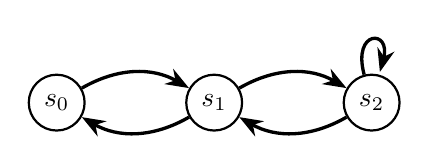
\begin{tikzpicture}
\begin{scope}[every node/.style={circle,thick,draw}]
    \node (s0) at (0,0) {$s_0$};
    \node (s1) at (2,0) {$s_1$};
    \node (s2) at (4,0) {$s_2$};
\end{scope}

\begin{scope}[>={Stealth[black]},
              every node/.style={fill=white,circle},
              every edge/.style={draw=black,very thick}]
    \path [->] (s0) edge[bend left=30] (s1);
    \path [->] (s1) edge[bend left=30] (s0);
    \path [->] (s1) edge[bend left=30] (s2);
    \path [->] (s2) edge[bend left=30] (s1);
    \path [->] (s2) edge[loop above] (s2);
\end{scope}
\end{tikzpicture}
\end{center}
Identify the set of states that satisfy each of the following and justify your answer:
\begin{enumerate}
\item $\ag{p} =\{ \}$
\item $\af{p}= \{s_0, s_1, s_2\}$
\item $\ag{\af{p}} = \{s_0, s_1, s_2\}$
\item $\af{\ag{p}} = \{ \}$  
\end{enumerate}
\hfill(2+2+3+3 pts)

\item Express the following statements as CTL formula:
\begin{enumerate}

\item
  There exists an execution sequence such that from every configuration in the sequence,
  it is possible to eventually satisfy the property $p$.
  
\textbf{Answer}: $\eg{\ef{p}}$
\item
  Along all paths, whenever $p$ is true, it is followed by a state where $p$ is false, and
  whenever $p$ is false, it is followed by a state where $p$ is true.
  
\textbf{Answer}:  $\ag{(p\rightarrow \ax{\neg p}) \land (\neg p \rightarrow \ax{p})}$
\end{enumerate}
\hfill (4+4 pts)

\item Prove or disprove the following:
  \begin{enumerate}
  \item
    If a state satisfies $\af{\ag{p}}$ then along all paths from that state the property $p$
    holds infinitely often.

    \textbf{Answer}: Let's assume, $$s_0 \in [[\af{\ag{p}}]]$$

    $$ \Rightarrow \forall \pi \in Path(s_0). \exists i \geq 0 \; \pi(i) \in [[\ag{p}]]$$
    $$ \Rightarrow \forall \pi \in Path(s_0). \exists i \geq 0 \; \pi(i) [ \forall \pi^\prime \in Path(\pi(i))\; \forall j >=i \; \pi^\prime(j) \in [[p]] ]$$
   This simplification tells that in all evaluations starting from the initial state, there exists a state from where $p$ holds in all paths globally. However, the question asks whether this CTL formula satisfies $p$
    holds infinitely often. Since $p$ holds globally in all paths, $\af{\ag{p}}$ disproves the property $p$
    holds infinitely often. 

    \item
    If a state satisfies $\af{\ag{p}}$ then along all paths from that state the property $\neg p$
    holds finitely many times. 
            
\textbf{Answer}: It is immediate from the previous question's explanation that, $\af{\ag{p}}$ does not hold $\neg p$ finitely many times, because the value of $i$ might be anything greater than 0. If $i$ becomes 0,  $\ag{p}$ holds from the initial state. Therefore, $\af{\ag{p}}$ does not ensure $\neg p$ holds finitely many times. 

  \item  If a state satisfies $\eg{\ef{p}}$ then there exists at least one path starting from that
    state where $p$ holds infinitely often.
    
\textbf{Answer}:
Let's assume, $$s_0 \in [[\eg{\ef{p}}]]$$

$$ \Rightarrow \exists \pi \in Path(s_0) \forall i \geq 0 \; \pi(i) \in [[\ef{p} ]]$$
$$\Rightarrow \exists \pi \in Path(s_0) \forall i \geq 0 \; \pi(i) [ \exists \pi^\prime \in Path(\pi(i)) \exists j \geq i \; \pi^\prime(j) \in [[p]]]$$

This implies that there exists a path that satisfies $p$ infinitely often. 
  
  \item $\au{p}{\ax{q}}$ is equivalent to $p \land \ax{\au{p}{q}}$

  \textbf{Answer}: Let's simplify  $\au{p}{\ax{q}}$ and $p \land \ax{\au{p}{q}}$ first. 

  We know $\au{\varphi}{\psi}$ can be written as $\psi \lor (\varphi \land \ax{\au{\varphi}{\psi}})$. So, we can write, $\au{p}{\ax{q}} \Leftrightarrow \ax{q} \lor (p \land \ax{\au{p}{\ax{q}}})$. We can claim a state $s$ satisfies $\au{p}{\ax{q}}$ if it satisfies either $\ax{q}$ or $p \land \ax{\au{p}{\ax{q}}}$. 
  
  
  % For the sake of simplicity, let's assume, $s$ only satisfies $\ax{q}$. We can write it as 
  % $$\forall s, s\in [[\ax{q}]] \Leftrightarrow \forall \pi \in Path(s): \pi(1) \in [[q]]$$

    Similarly, $$p \land \ax{\au{p}{q}} \Leftrightarrow p \land \ax{q \lor (p \land \ax{\au{p}{q}})}$$
   
    % Now let's assume $q$ is satisfied from $q \lor (p \land \ax{\au{p}{q}})$. Then we can write 

    % $$p \land \ax{\au{p}{q}} \Leftrightarrow p \land \ax{q}$$
    
    % We can further write it as follows-

    %   $$\forall s, s\in [[p \land \ax{q}]] \Leftrightarrow \forall \pi \in Path(s): \pi(0) \in [[p]] \land \pi(0) \in [[\ax{q}]]$$

Now, construct a Kripke structure satisfying $\au{p}{\ax{q}}$. 


  \begin{center}
  \begin{tabular}{cc}
  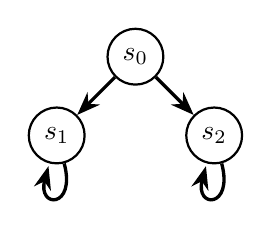
\begin{tikzpicture}
\begin{scope}[every node/.style={circle,thick,draw}]
    \node (s0) at (0,0) {$s_0$};
    \node (s1) at (-1,-1) {$s_1$};
    \node (s2) at (1,-1) {$s_2$};
\end{scope}

\begin{scope}[>={Stealth[black]},
              every node/.style={fill=white,circle},
              every edge/.style={draw=black,very thick}]
    \path [->] (s0) edge (s1);
    \path [->] (s0) edge  (s2);
    \path [->] (s1) edge[loop below] (s1);
    \path [->] (s2) edge[loop below] (s2);
\end{scope}
  \end{tikzpicture}
  &
  %%
  \begin{tabular}{l}
    $L(s_1) = \{q\}$, $L(s_2) = \{q\}$
    \end{tabular}
  \end{tabular}
\end{center}

From the above simplification, we know the above Kripke structure satisfies $\au{p}{\ax{q}}$ because it holds $\ax{q}$. However, it does not satisfy $p \land \ax{\au{p}{q}}$ because it requires $p$ to be true at the initial state.  
  
Therefore, we can say that $\au{p}{\ax{q}}$ is not equivalent to $p \land \ax{\au{p}{q}}$.

    
  \item \emph{For 512. Extra credit for 412 students}
    The property, \emph{for all paths of the form $\pi$, $p$ is true in every $\pi[i]$ where $i$ is even},
    can be expressed in CTL.
    
    \textbf{Answer}: Let's consider a infinite path $\pi = s_0, s_1, s_2, ..., s_n, s_{n+1}, ... s_{n+k}, ...$. 

    Here $\pi[i] \in [[p]]$ when $i=\{0, 2, 4, 6, 8, ... \}$, and all the odd position $\pi[i] \in [[ \neg p]]$ where $i = \{ 1,3,5,7, ...\}$. 

    The traces of the paths, $traces(\pi)= \{p, \neg p, p, \neg p, p, \neg p, ... \}$. As all the paths follow the same forms, we can say that $p$ is repeated infinitely often. Therefore, we can write it as $\ag{\af{p}}$, which is a valid CTL formula. 
    
  \end{enumerate}
  \hfill (2+2+3+3+4 pts)
  
\end{enumerate}


\end{document}

